\tableofcontents
\pagebreak

\section{Свободное движение}
Рассмотрим систему второго порядка в форме В-В:
\begin{equation}
    \ddot{y} + a_1 \dot{y} + a_0 y  = u
\end{equation}
Согласно заданию, выберем три набора корней $(\lambda_1, \lambda_2)$, удовлетворяющих модам из задания (2,3,8)
и найдем небходимы пары коэффициентов $(a_1, a_0)$:
\begin{enumerate}
    \item Нейтральная и устойчивая апериодическая: $\lambda_1 = 0, \lambda_2 = -1$; $a_1 = 1, a_0 = 0$
    \item Нейтральная и неустойчивая апериодическая: $\lambda_1 = 0, \lambda_2 = 0.3$; $a_1 = -0.3, a_0 = 0$
    \item Пара неусточивых колебательных мод: $\lambda_1 = 0.4 + 2i, \lambda_2 = 0.4 - 2i$; $a_1 = -0.8, a_0 = 4.16$
\end{enumerate}


\begin{figure}[h]
    \centering
    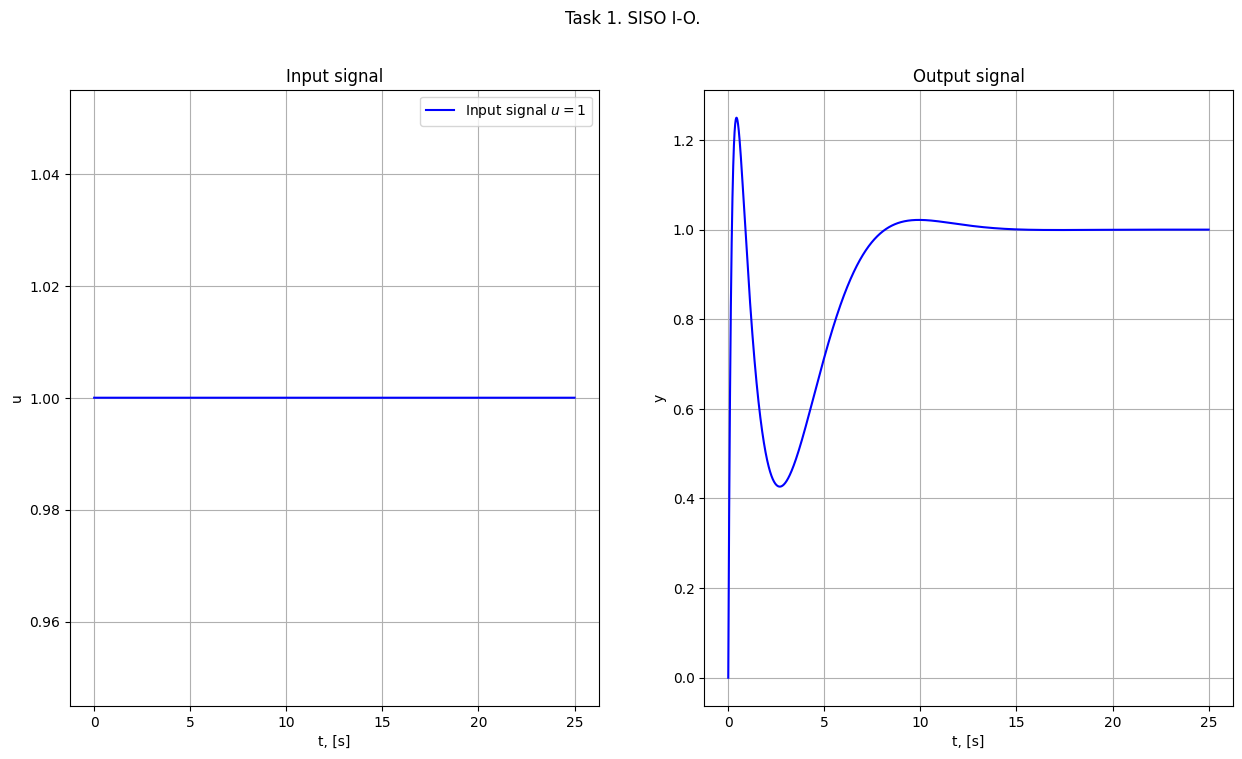
\includegraphics[width=\textwidth]{plot_1_1}
    \caption{\label{fig:The-caption-1}Входные и выходные сигналы систем при нулевых начальных условиях (задание 1)}
\end{figure}

Вычисления пары $(a_1, a_0)$ проведем, воспользовавшись теоремой Виета:
\begin{equation*}
    \begin{cases}
        \lambda_1 + \lambda_2 = - a_1 \\
        \lambda_1 \lambda_2 = a_0
    \end{cases}
\end{equation*}
Согласно корневому критерию, первый набор корней соответствует апериодической системе на границе 
 устойчивости (оба корня действительные, неотрицательны и не кратные), второй - неустойчивой 
 апериодической системе (корни действительные, один из корней имеет положительную действительную часть),
 третий - неустойчивой колебательной системе (пара комплексно сопряженных корней с положительной 
 действительной частью).

 Проведем моделирование поведения систем с нулевыми начальными условиями и при $y(0)=0, \dot y (0) = 1$ 
 (рис. 1 и рис. 2 соответственно).
 

 \begin{figure}[h]
    \centering
    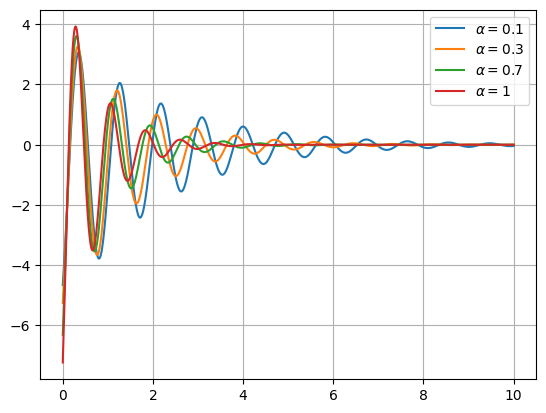
\includegraphics[width=\textwidth]{plot_1_2}
    \caption{\label{fig:The-caption-1}Входные и выходные сигналы систем при ненулевых начальных условиях (задание 1)}
\end{figure}

Заметим, что все системы ведут себя одинаково при задании нулевых начальных условий 
и подаче нулевого управляющего воздействия (они статичны в 0). При задании начальных условий системы
ведут себя согласно аналитически предсказанному корневым критерием.

\pagebreak

\section{Область устойчивости}
Рассмотрим систему, заданную следующей блок-схемой:
\begin{figure}[h]
    \centering
    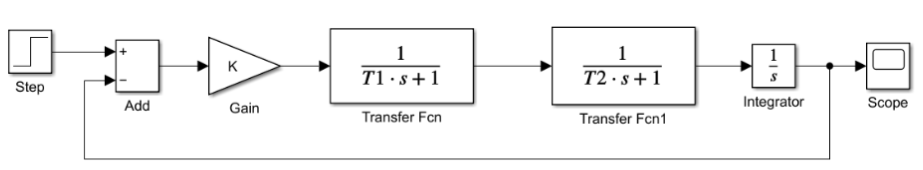
\includegraphics[width=\textwidth]{pic_2_0}
\end{figure}

Можем представить систему передаточной функцией:
\begin{equation*}
    W_0(s) = K, W_1(s) = \frac{1}{T_1 s + 1}, W_2(s) = \frac{1}{T_2 s + 1}, W_3(s)=\frac{1}{s} 
\end{equation*}
\begin{equation*}
    y = W_0W_1W_2W_3(s)[u - y] \implies y = \frac{W_0W_1W_2W_3}{1 + W_0W_1W_2W_3}(s)[u], y = W(s)[u]
\end{equation*}
\begin{equation}
    W(s)=\frac{\frac{K}{s(T_1 s + 1)(T_2 s + 1)}}{1 + \frac{K}{s(T_1 s + 1)(T_2 s + 1)}}=
    \frac{K}{s(T_1 s + 1)(T_2 s + 1) + K}=\frac{K}{T_1 T_2 s^3 + (T_1 + T_2) s^2 + s + K}
\end{equation}
Первый набор корней из первого задания: $\lambda_1 = 0, \lambda_2 = 1$. Таким образом, мы 
не можем выбрать $T_1$. Система с передаточной функцией $\frac{\frac{K}{T_2}}{s^3 + \frac{1}{T_2}s^2 + \frac{K}{T_2}}$
не может быть асимптотически устойчивой согласно критерию Гурвица т.к. условие $a_1 = 0 > 0$ не может быть выполнено.
Граница устойчивости достигается при любом $T_2 \ge 0$ и $K=0$.
Для анализа системы на устойчивость возьмем $\lambda_1 = 1, \lambda_2 = -1$, тогда $T_1=-1, T_2=1$.

Зафиксируем $T_2 = 1$. Запишем критерий Гурвица:
\begin{equation*}
    W(s) = \frac{\frac{K}{T_1}}{s^3 + \frac{T_1 + 1}{T_1} s^2 + \frac{1}{T_1}s + \frac{K}{T_1}}
    \implies 
    \begin{cases}
        \frac{T_1 + 1}{T_1} > 0 \\
        \frac{1}{T_1} > 0 \\
        \frac{K}{T_1} > 0 \\
        \frac{T_1 + 1}{T_1 ^ 2} > \frac{K}{T_1}
    \end{cases} \implies
    \begin{cases}
        T_1 > 0 \\
        K > 0 \\
        K < 1 + \frac{1}{T_1}
    \end{cases}
\end{equation*}
Таким образом, зона устойчивости ограничена прямыми $K=0$, $T_1=0$ и гиперболой $K = 1 + \frac{1}{T_1}$ (рис. 3).

Зафиксируем $T_1 = -1$. Запишем критерий Гурвица:
\begin{equation*}
    W(s) = \frac{\frac{K}{T_2}}{s^3 + \frac{1 - T_2}{T_2} s^2 - \frac{1}{T_2}s - \frac{K}{T_2}}
    \implies 
    \begin{cases}
        \frac{1 - T_2}{T_2} > 0 \\
        -\frac{1}{T_2} > 0 \\
        -\frac{K}{T_2} > 0 \\
        \frac{T_2 - 1}{T_2 ^ 2} > -\frac{K}{T_2}
    \end{cases} \implies
    \begin{cases}
        T_2 < 0 \\
        K > 0 \\
        K < -1 + \frac{1}{T_2}
        % -\frac{T_2 - 1}{T_2 } > K 
    \end{cases} \implies \varnothing
\end{equation*}
Таким образом, система не имеет зоны устойчивости.

\begin{figure}[]
    \centering
    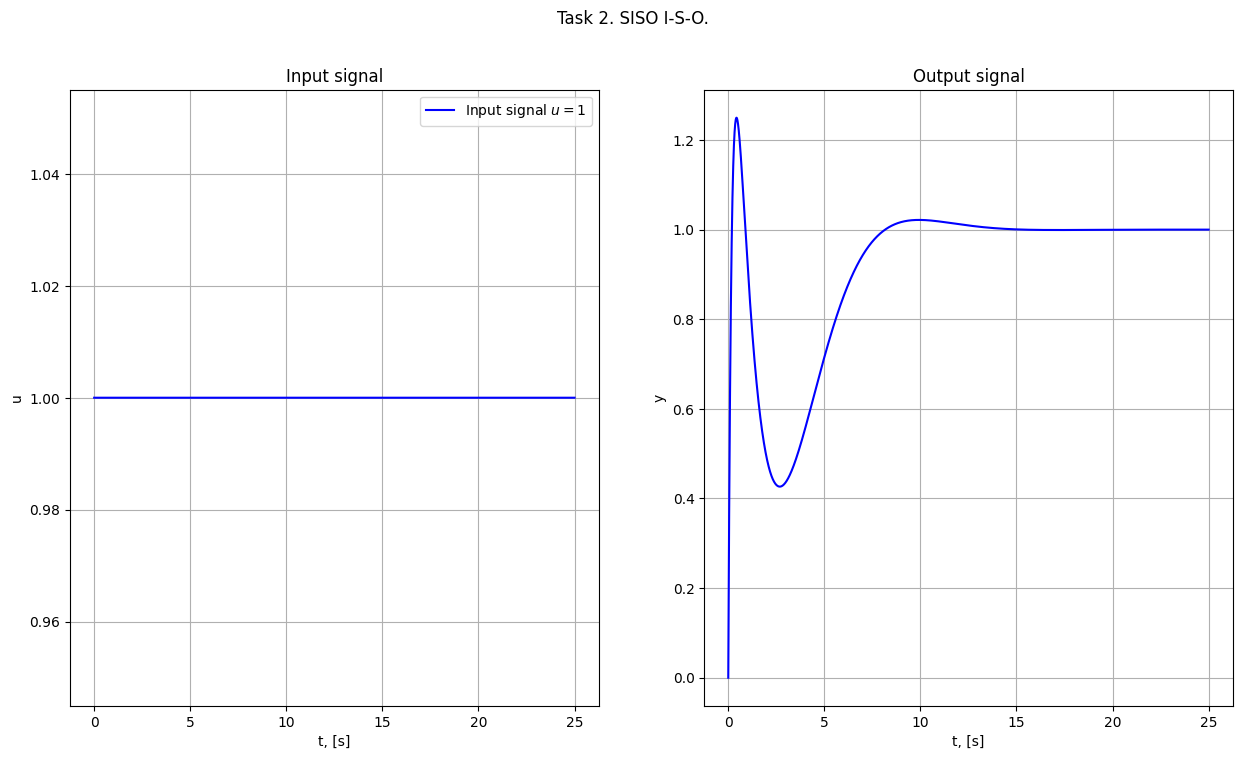
\includegraphics[width=\textwidth]{plot_2_1}
    \caption{\label{fig:The-caption-1}Зона устойчивости при фиксированном $T_2=1$ (задание 2)}
\end{figure}
\begin{figure}[]
    \centering
    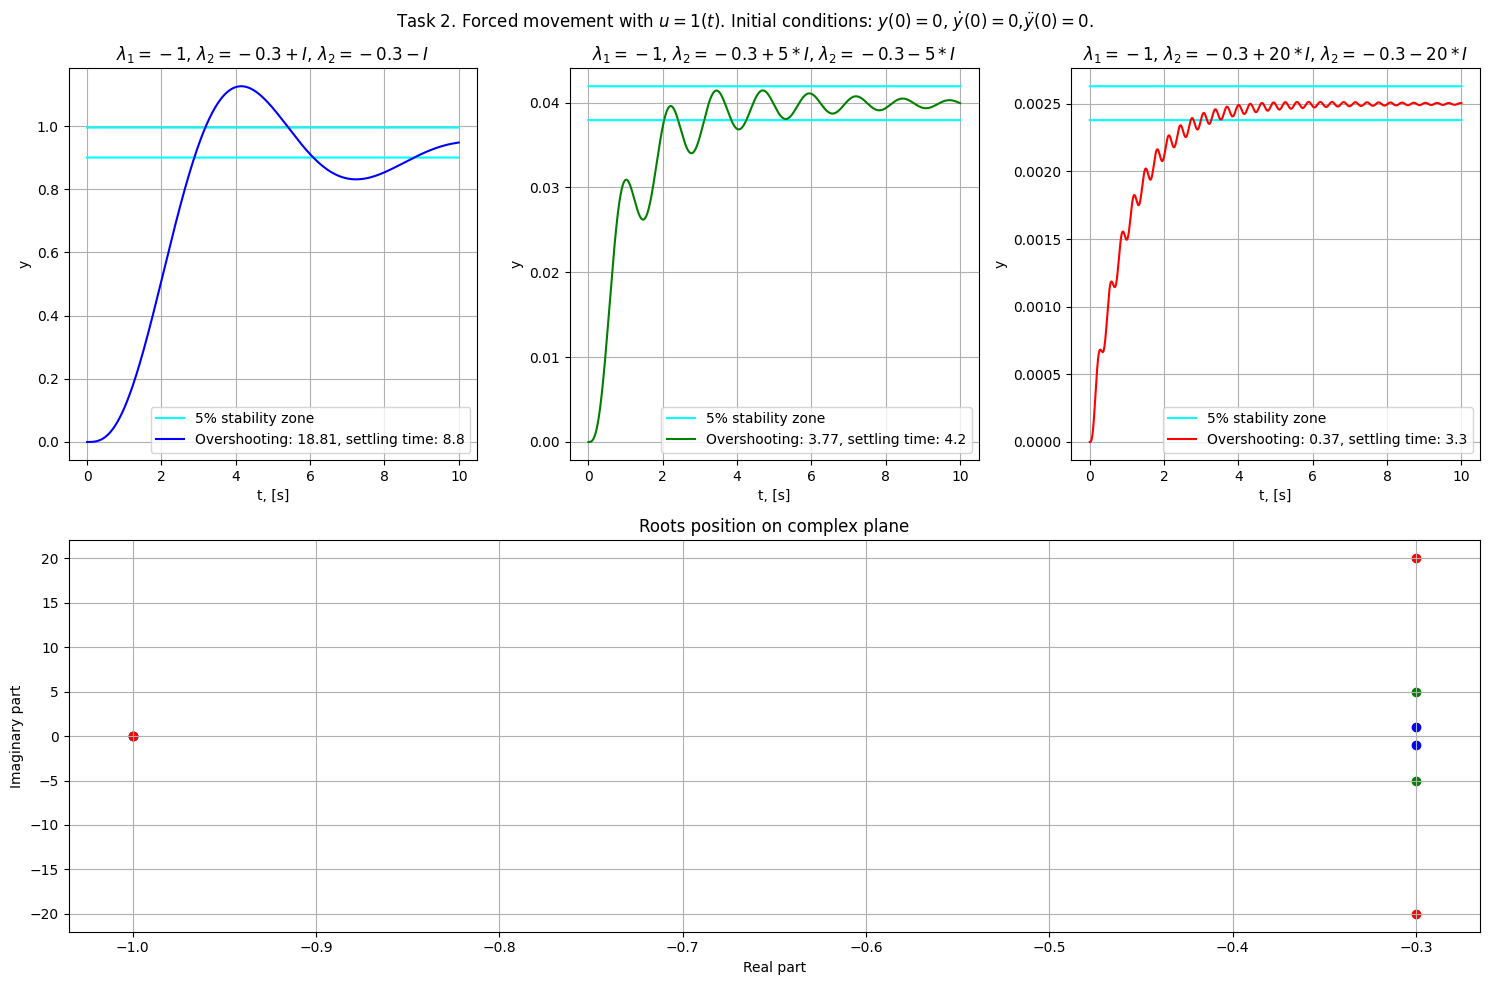
\includegraphics[width=\textwidth]{plot_2_2}
    \caption{\label{fig:The-caption-1}Моделирование систем с разными типами устойчивости (задание 2)}
\end{figure}
\pagebreak

\section{Автономный генератор}

\pagebreak

\section{Изучение канонической управляемой формы: фазовые портреты}

\pagebreak